\paragraph{问题与可比证据。}
地形分支考察拟合地图修正是否改善其纯历史base，不是普通HSM-SDE与CV的比较。
十个配置均已拟合并执行预测。原主网格包含2,300个不同槽位：2,297成功、三个失败，
没有待运行或缺失槽位。为比较相同观测，本文描述十配置、五种子全部成功的43个记录块交集，
共2,150槽位。三个完整记录块被排除于这项事后比较；失败值不填零，也不替换。
筛选依据执行状态而不是哪个模型更好，但仍以执行成功为条件。
这些汇总不估计原完整46块总体的表现，不替代登记推断。
先在块内平均五种子，再对块等权汇总；所有底层评分和预测均未改变。

\paragraph{整体组合：描述性汇总没有收益。}
共同子集上，全地形平均ES为482.06米，base为455.08米，变化$+26.98$米；
FDE为1459.37对1420.37米，变化$+39.00$米（表\ref{tab:terrain-description}）。
全地形四个目标的ES均更高，30分钟差为$+69.11$米（图\ref{fig:terrain-description}）。
但全地形在43块中的22块平均ES更低，因此总体均值劣势与局部收益可以并存；
选出的成功案例地图不能建立平均地形收益。
这是该拟合组合在所选子集上的描述结果，不是显著有害判断，也不证明地形信息本身没有价值。

\begin{table}[!htbp]\centering
\caption{相同43个完整记录块的地形预测（每块五种子）。ES平均四目标，$\Delta$ES均相对base；FDE、覆盖和面积取30分钟。成功数保留各配置原230槽位分母。这是事后描述均值，不是登记完整家族效应。}\label{tab:terrain-description}
\small\setlength{\tabcolsep}{3pt}
\begin{tabular}{lrrrrrr}\toprule
配置 & ES（米） & $\Delta$ES（米） & FDE（米） & 覆盖（\%） & 面积（km$^2$） & 成功数\\\midrule
base & 455.08 & +0.00 & 1420.37 & 46.05 & 5.503 & 230/230\\
all-terrain & 482.06 & +26.98 & 1459.37 & 40.47 & 5.609 & 229/230\\
lio-road & 498.04 & +42.96 & 1493.33 & 52.09 & 6.202 & 229/230\\
lio-river & 455.27 & +0.19 & 1478.38 & 41.40 & 5.701 & 229/230\\
lio-worldcover & 453.44 & -1.64 & 1414.40 & 49.77 & 5.635 & 230/230\\
lio-surface & 462.66 & +7.58 & 1410.27 & 47.44 & 5.670 & 230/230\\
loo-road & 462.19 & +7.11 & 1459.69 & 44.65 & 5.719 & 230/230\\
loo-river & 498.29 & +43.20 & 1446.22 & 50.23 & 5.693 & 230/230\\
loo-worldcover & 482.14 & +27.06 & 1465.55 & 41.40 & 5.886 & 230/230\\
loo-surface & 477.11 & +22.03 & 1485.96 & 46.51 & 6.145 & 230/230\\
\bottomrule\end{tabular}
\end{table}

\begin{figure}[!htbp]\centering
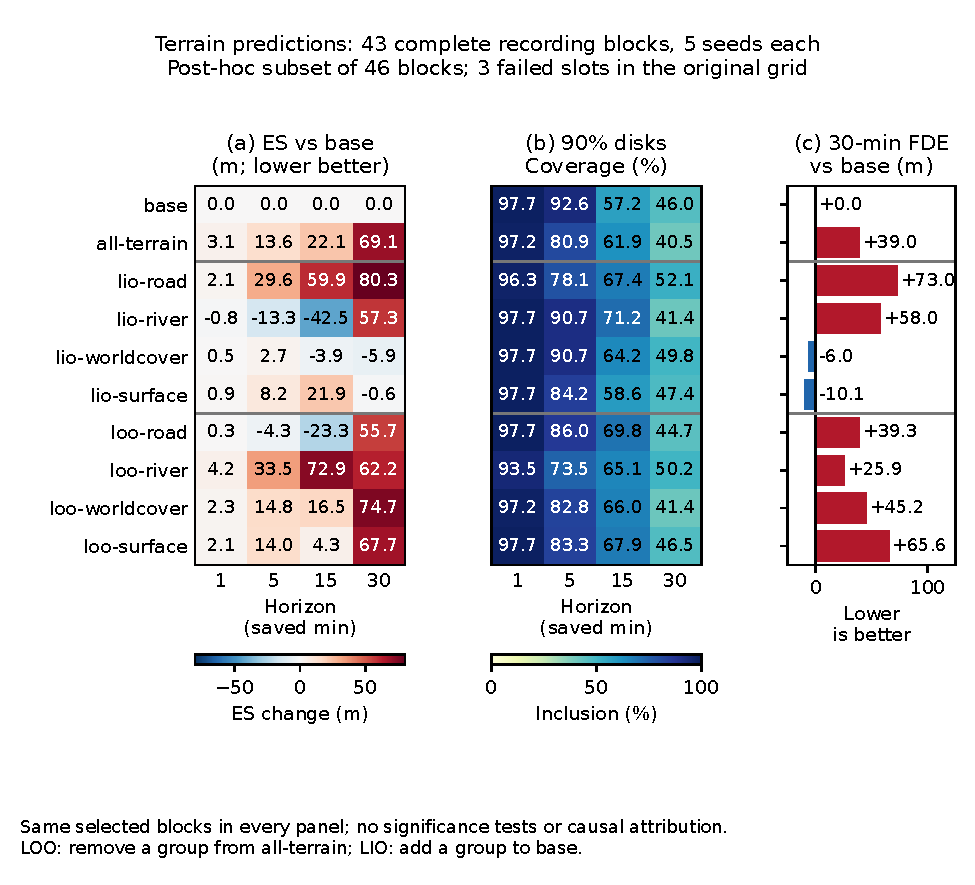
\includegraphics[width=\linewidth]{../figures/terrain-description-v1/terrain-evidence.pdf}
\caption{已有地形预测在同一事后43块子集上的比较。左：四时域相对纯历史base的ES差，
负值有利；中：名义90\%圆的实际包含率，校准目标是90\%；右：30分钟预测均值误差相对base的差。
各面板使用相同记录块，均先平均五种子再等权平均块。LIO向base加入一组，
LOO从全地形移除一组及依赖交互。比较对象是配置表现，不是隔离的因素效应。
表\ref{tab:terrain-description}保留完整网格失败分母；不提供推断区间。}
\label{fig:terrain-description}\end{figure}

\paragraph{因素配置：组合背景与时域均重要。}
仅加入道路组相对base使平均ES增加42.96米，从全地形移除道路则使ES下降19.87米。
两个方向都将当前道路表示与这些拟合配置中的评分代价联系起来，
不能推广为道路不能帮助预测。仅河流相对base使15分钟ES下降42.51米，
30分钟却增加57.27米，平均ES仅变化$+0.19$米；
从完整组合移除河流却使平均ES增加16.22米。
因此单独加入的表现不能决定一个因素在完整组合中的作用。

仅地表覆盖配置的平均ES为453.44米，在十个保存配置均值中最低，
但相对base的改善只有1.64米，FDE降低5.96米。
仅坡面配置则使平均ES增加7.58米、FDE降低10.09米。
二者分别说明小幅有利配置及评分--定位取舍，不能据此确认某个因素优越。
配置间拟合、扩散、交互及有效正则化同时改变，差异不能归为单个地形因素的因果效应。

\paragraph{更大配对子集与区域可靠性。}
描述性敏感性核查进一步保留每候选／对照对所有五种子完整块：涉及失败配置的比较为45块，
完整单组／base比较为46块。此时全地形／base的ES差为$+21.17$米，
仅道路／base为$+41.18$米，移除道路为$-18.50$米，仅地表覆盖／base为$-3.81$米，
方向与共同子集一致。仅河流／base却从$+0.19$变为$-1.54$米，说明接近零的平均结果脆弱。
较大子集同样以成功为条件，使用不同记录块，不能恢复缺失的完整队列估计目标或支持全局排名。

共同子集十配置的30分钟名义90\%覆盖仅为40.47--52.09\%。
全地形为40.47\%，base为46.05\%，尽管全地形平均面积略大：5.609对5.503平方千米。
因此本次比较中，地形条件化没有使长时域预测圆具有经验可靠性。
已有数据整体显示配置和时域依赖的取舍，而非加入全部地形组的一致收益。
原登记完整家族回答仍按下列规则单独保持不可用。
